\subsection{Dataset}
The prepared dataset contained 11,111 unique publication documents from 3,257 researchers, split into 2,605 training and 652 test researchers. Fig.~\ref{fig:dataset}(a) showed large differences in group membership: Machine Learning was largest (2,480 researchers), followed by Artificial Intelligence (2,090) and Computer Vision (1,748), while Visualization (118) and Software Engineering (127) were smallest; counts exceed the number of unique researchers because one researcher could belong to several groups. Publication profile size was also uneven (Fig.~\ref{fig:dataset}(b)): a mean of 6.1 publications per researcher and a median of 2, ranging from 1 to 59, with the gap between mean and median and the long right tail showing that most researchers had short profiles while a smaller number had many.

Fig.~\ref{fig:dataset}(c) described the multi-label structure of the task: only 421 researchers (13\%) belonged to one group, membership in three groups was most common (703 researchers, 22\%), two and four groups accounted for about 18\% and 20\%, and the remainder belonged to five or more groups, including nine researchers with nine labels -- representing researcher placement as a ranked multi-group problem rather than single-label classification.

\begin{figure}[t]
    \centering
    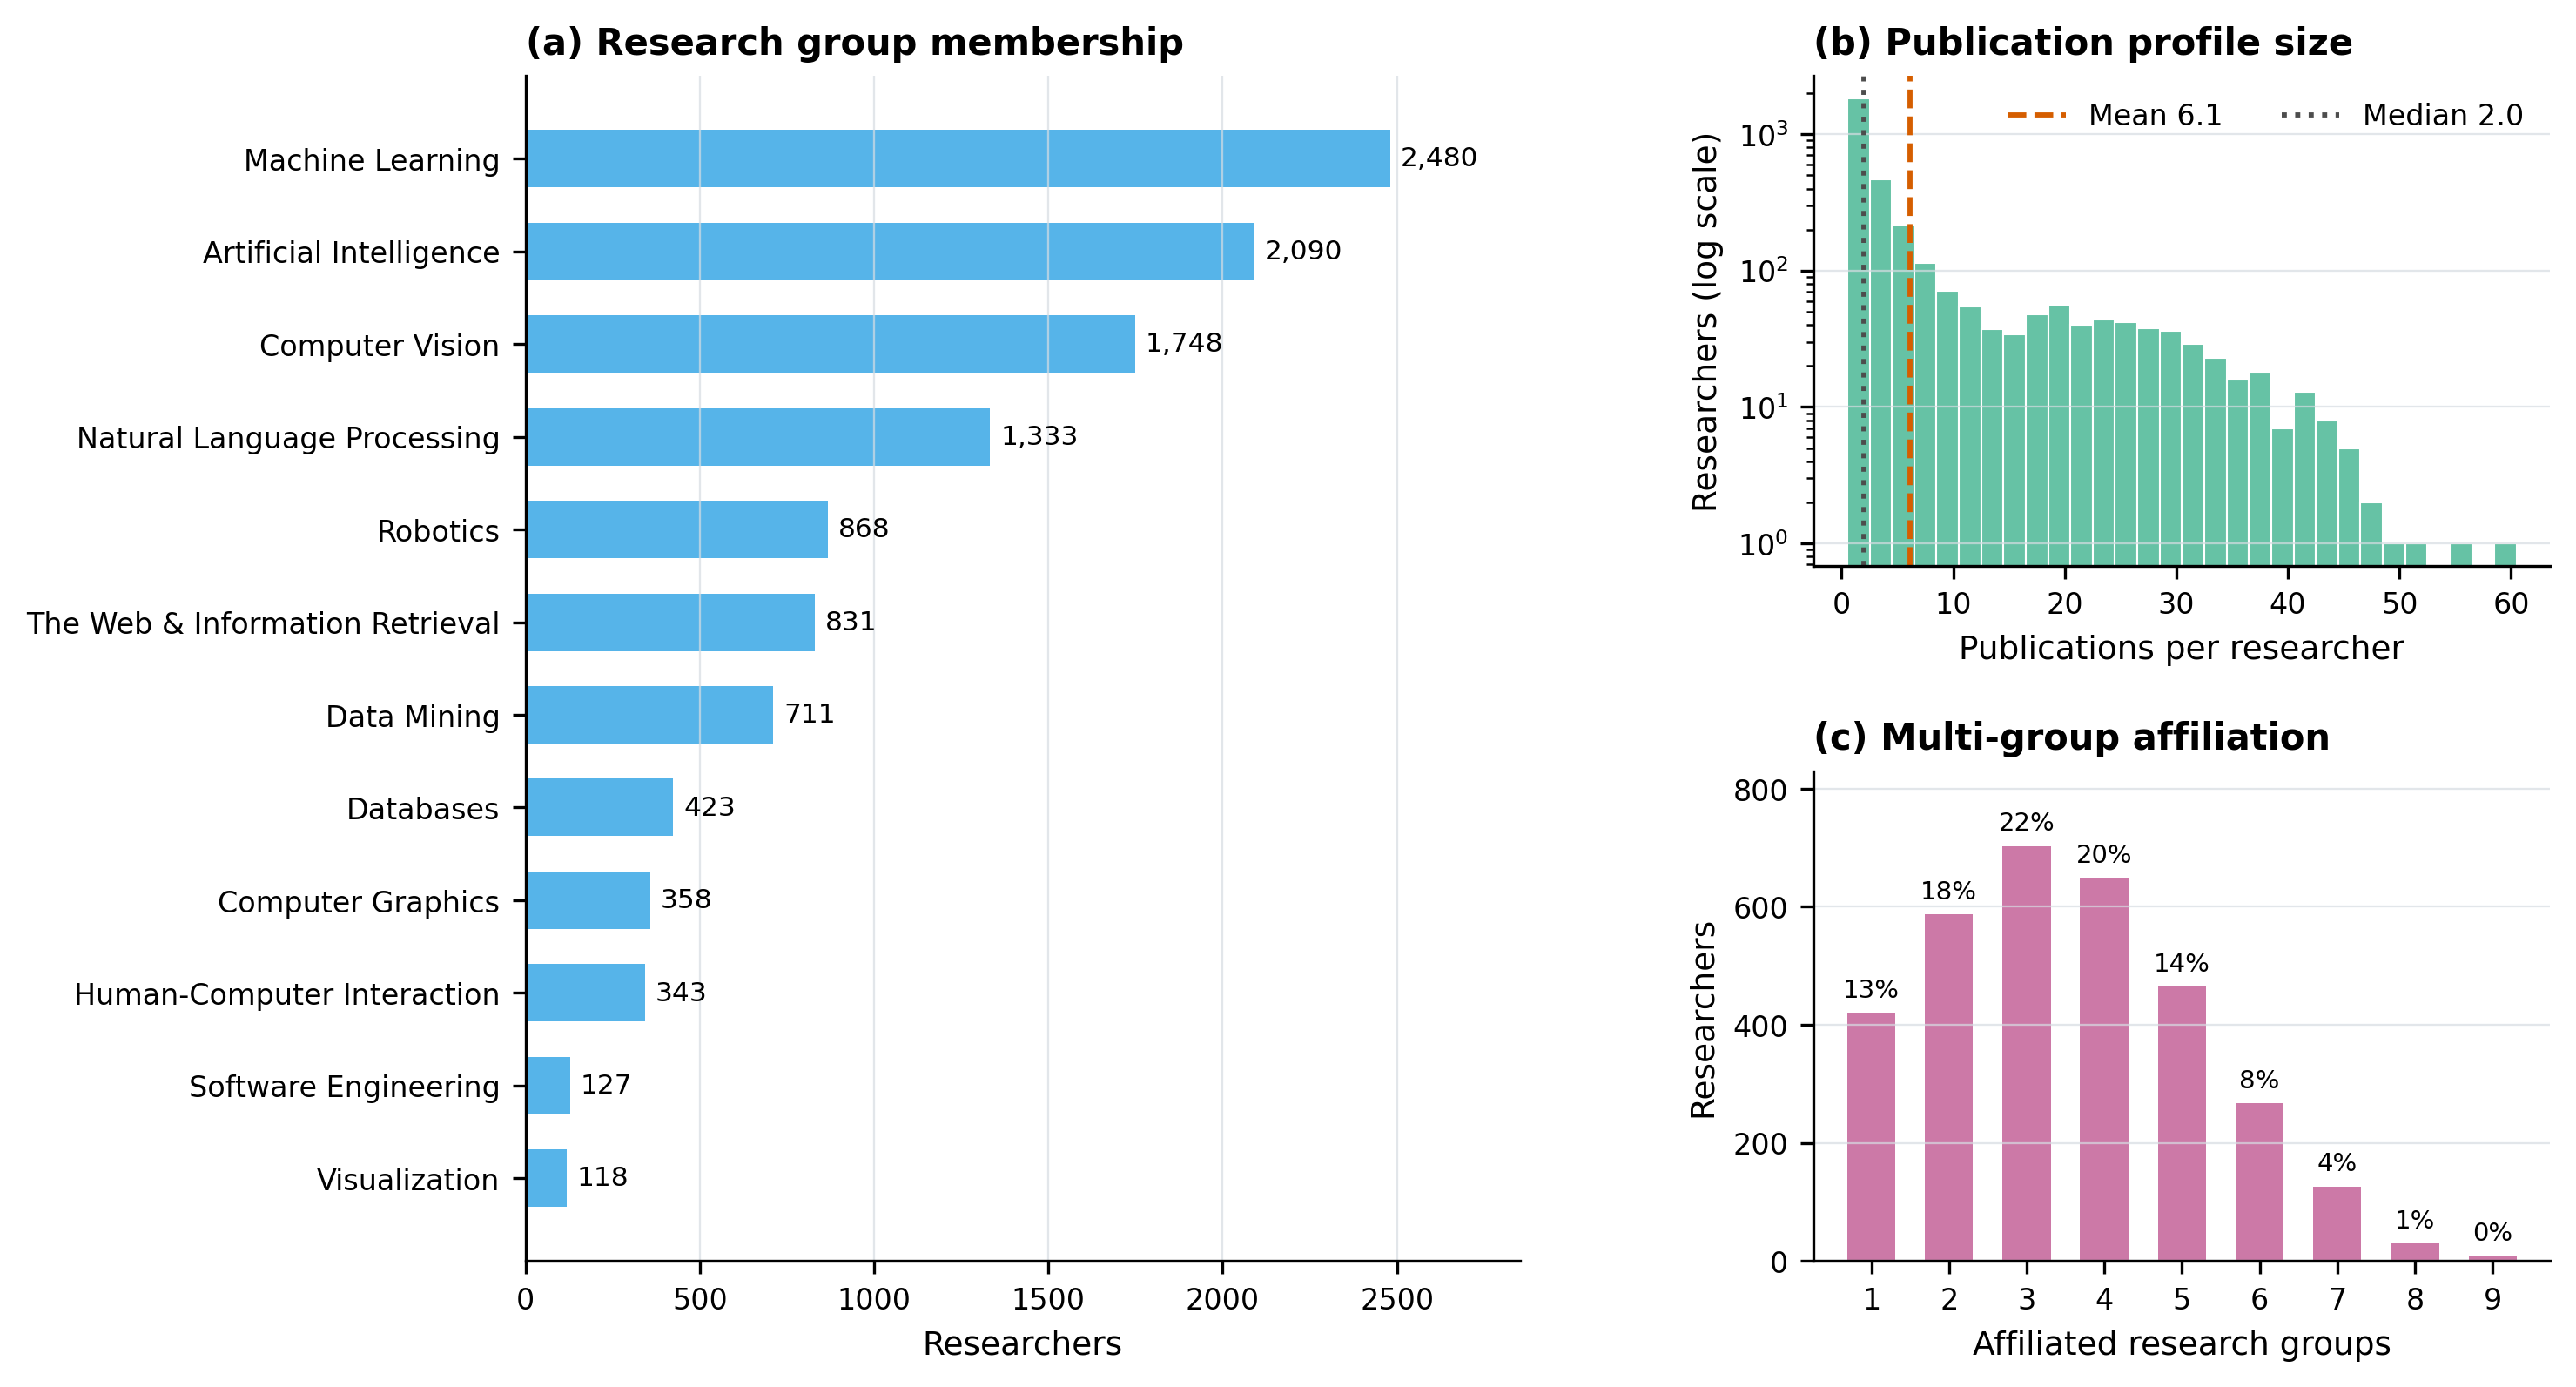
\includegraphics[width=0.94\columnwidth]{sections/figures/02_dataset_characterization.png}
    \caption{Dataset characteristics: (a) researcher membership in each group, (b) the distribution of publication profile sizes, and (c) the number of research group affiliations per researcher.}
    \label{fig:dataset}
\end{figure}

\subsection{Hyperparameter Optimization}
Fig.~\ref{fig:hpsearch} reported the training-corpus $C_v$ coherence obtained during the parameter search. For LDA, the highest coherence (0.521625) was obtained with 29 topics, against 0.512700--0.518153 for the other three tested counts. For NMF, the best configuration (11 topics) reached 0.686782, against 0.683174 for 9 topics and lower values for 12 and 15. The BERTopic search covered nine combinations of minimum topic size and UMAP neighbors: a minimum topic size of 45 with 50 neighbors ranked first (0.659480, 43 topics), close to 45/55 neighbors (0.658543), while two configurations at 60 neighbors produced only five topics and the lowest coherence (0.533384); all configurations reported zero remaining noise documents after outlier reassignment. The rank-one configuration for each model was used in the final experiment.

\begin{figure}[t]
    \centering
    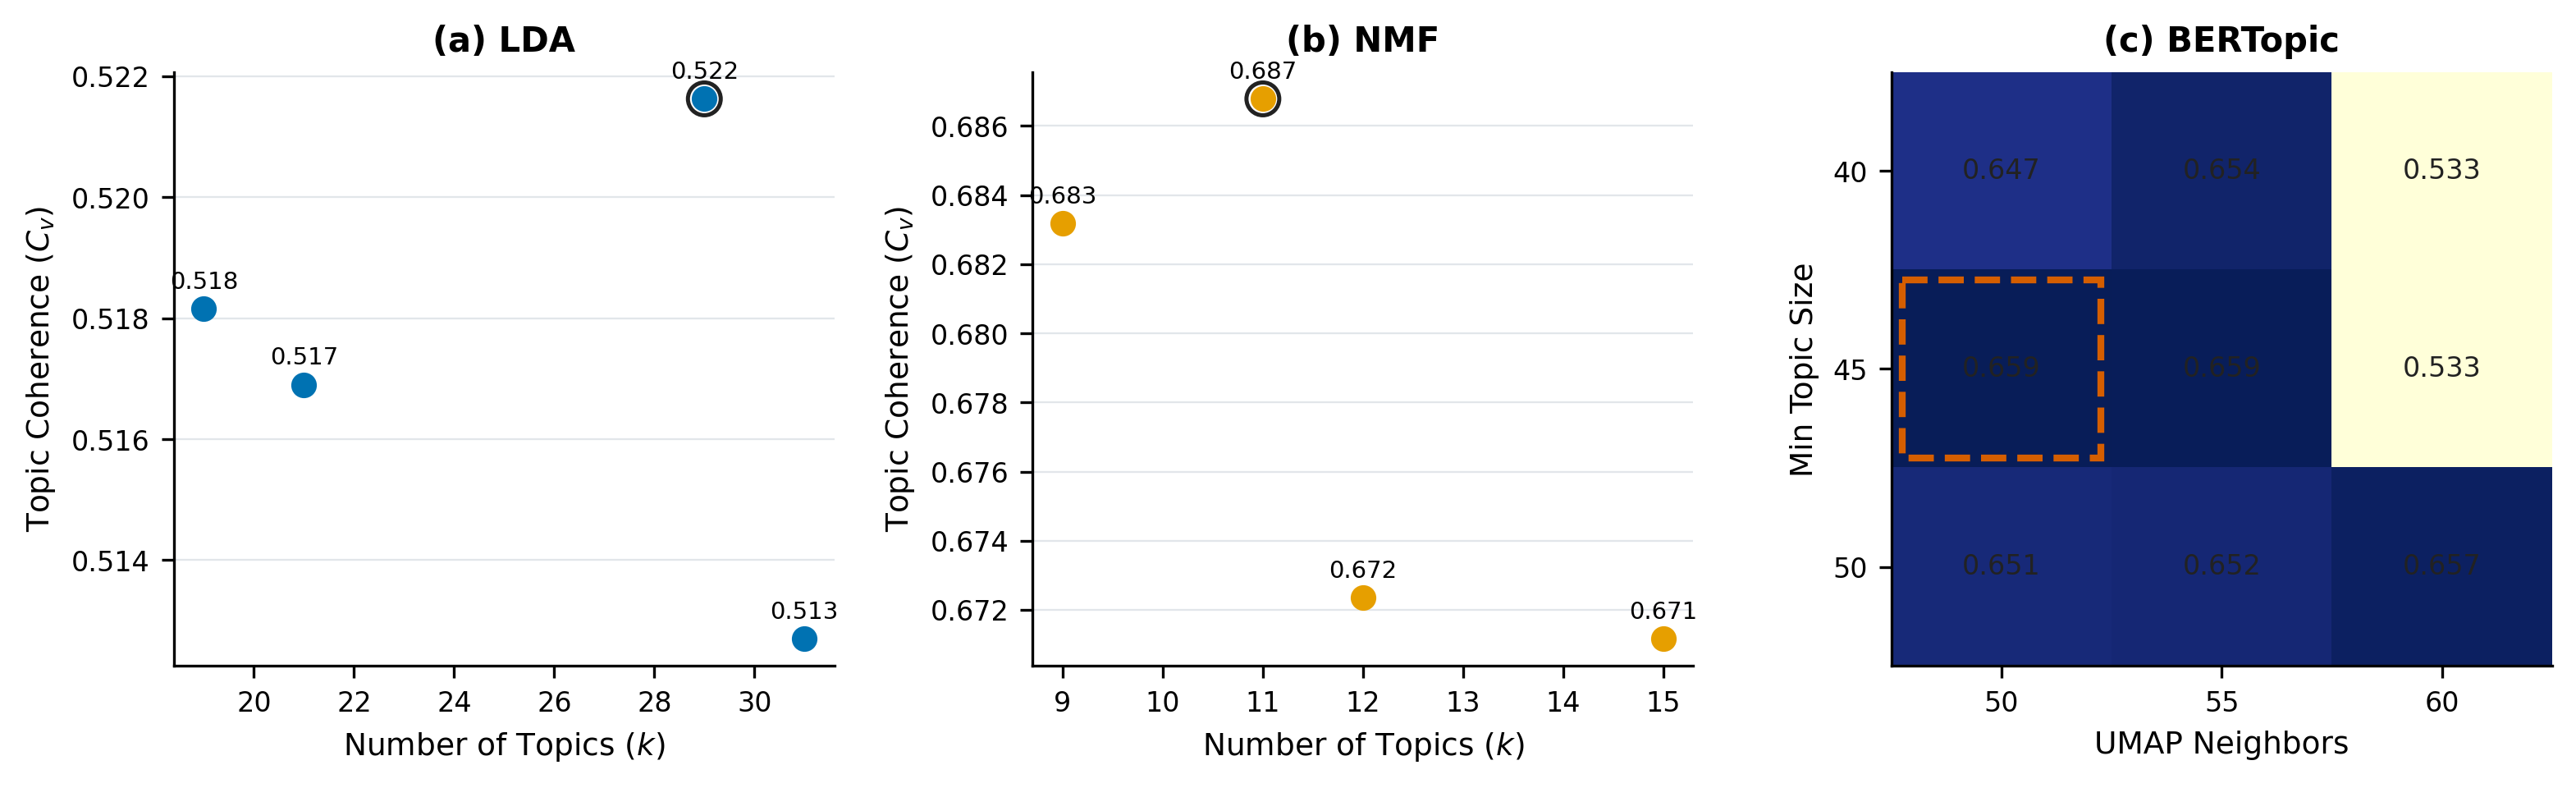
\includegraphics[width=0.94\columnwidth]{sections/figures/03_hyperparameter_search.png}
    \caption{Training-corpus hyperparameter search.}
    \label{fig:hpsearch}
\end{figure}

\subsection{Recommendation Performance}
Table~\ref{tab:main} summarizes the main test results at $K=5$ and MRR, together with paired Wilcoxon signed-rank tests (Section~\ref{sec:sigtest}) against BERTopic. BERTopic obtained the highest value in every metric, reaching an NDCG@5 of 0.736 and MRR of 0.809 against 0.719/0.793 for LDA and 0.640/0.774 for NMF. Fig.~\ref{fig:recperf} extends the comparison to Precision, Recall, F1-score, and NDCG at $K=1,3,5$: BERTopic ranked first in all 12 cutoff-based metrics; Precision decreased and Recall increased as more groups were returned, F1-score rose because the gain in Recall exceeded the loss in Precision, and NDCG stayed above 0.60 for every model and cutoff. Across all 13 reported metrics, BERTopic ranked first, LDA second, and NMF third.

\begin{table}[t]
\caption{Recommendation Performance ($K{=}5$, MRR) and Paired Wilcoxon Tests vs.\ BERTopic (BT), $n=652$}
\label{tab:main}
\centering
\scriptsize
\setlength{\tabcolsep}{3pt}
\begin{tabular}{lrrrrrrr}
\toprule
 & & & & \multicolumn{2}{c}{BT$-$LDA} & \multicolumn{2}{c}{BT$-$NMF} \\
Metric & LDA & NMF & BT & $\Delta$ & $p$-value & $\Delta$ & $p$-value \\
\midrule
P@5    & 0.4966 & 0.4301 & 0.5080 & 0.0113 & 0.097 & 0.0779 & $<0.001^{*}$ \\
R@5    & 0.7647 & 0.6770 & 0.7824 & 0.0177 & 0.007$^{*}$ & 0.1054 & $<0.001^{*}$ \\
F1@5   & 0.5652 & 0.4923 & 0.5790 & 0.0138 & 0.007$^{*}$ & 0.0867 & $<0.001^{*}$ \\
NDCG@5 & 0.7199 & 0.6405 & 0.7362 & 0.0163 & 0.073 & 0.0957 & $<0.001^{*}$ \\
MRR    & 0.7932 & 0.7750 & 0.8093 & 0.0160 & 0.113 & 0.0343 & 0.003$^{*}$ \\
\bottomrule
\end{tabular}
\vspace{2pt}

\raggedright\scriptsize $^{*}$Significant at uncorrected $\alpha=0.05$. None of the BT-vs-LDA comparisons survive the Bonferroni threshold $\alpha\approx0.0038$ (13 tests); all BT-vs-NMF comparisons do.
\end{table}

\begin{figure}[t]
    \centering
    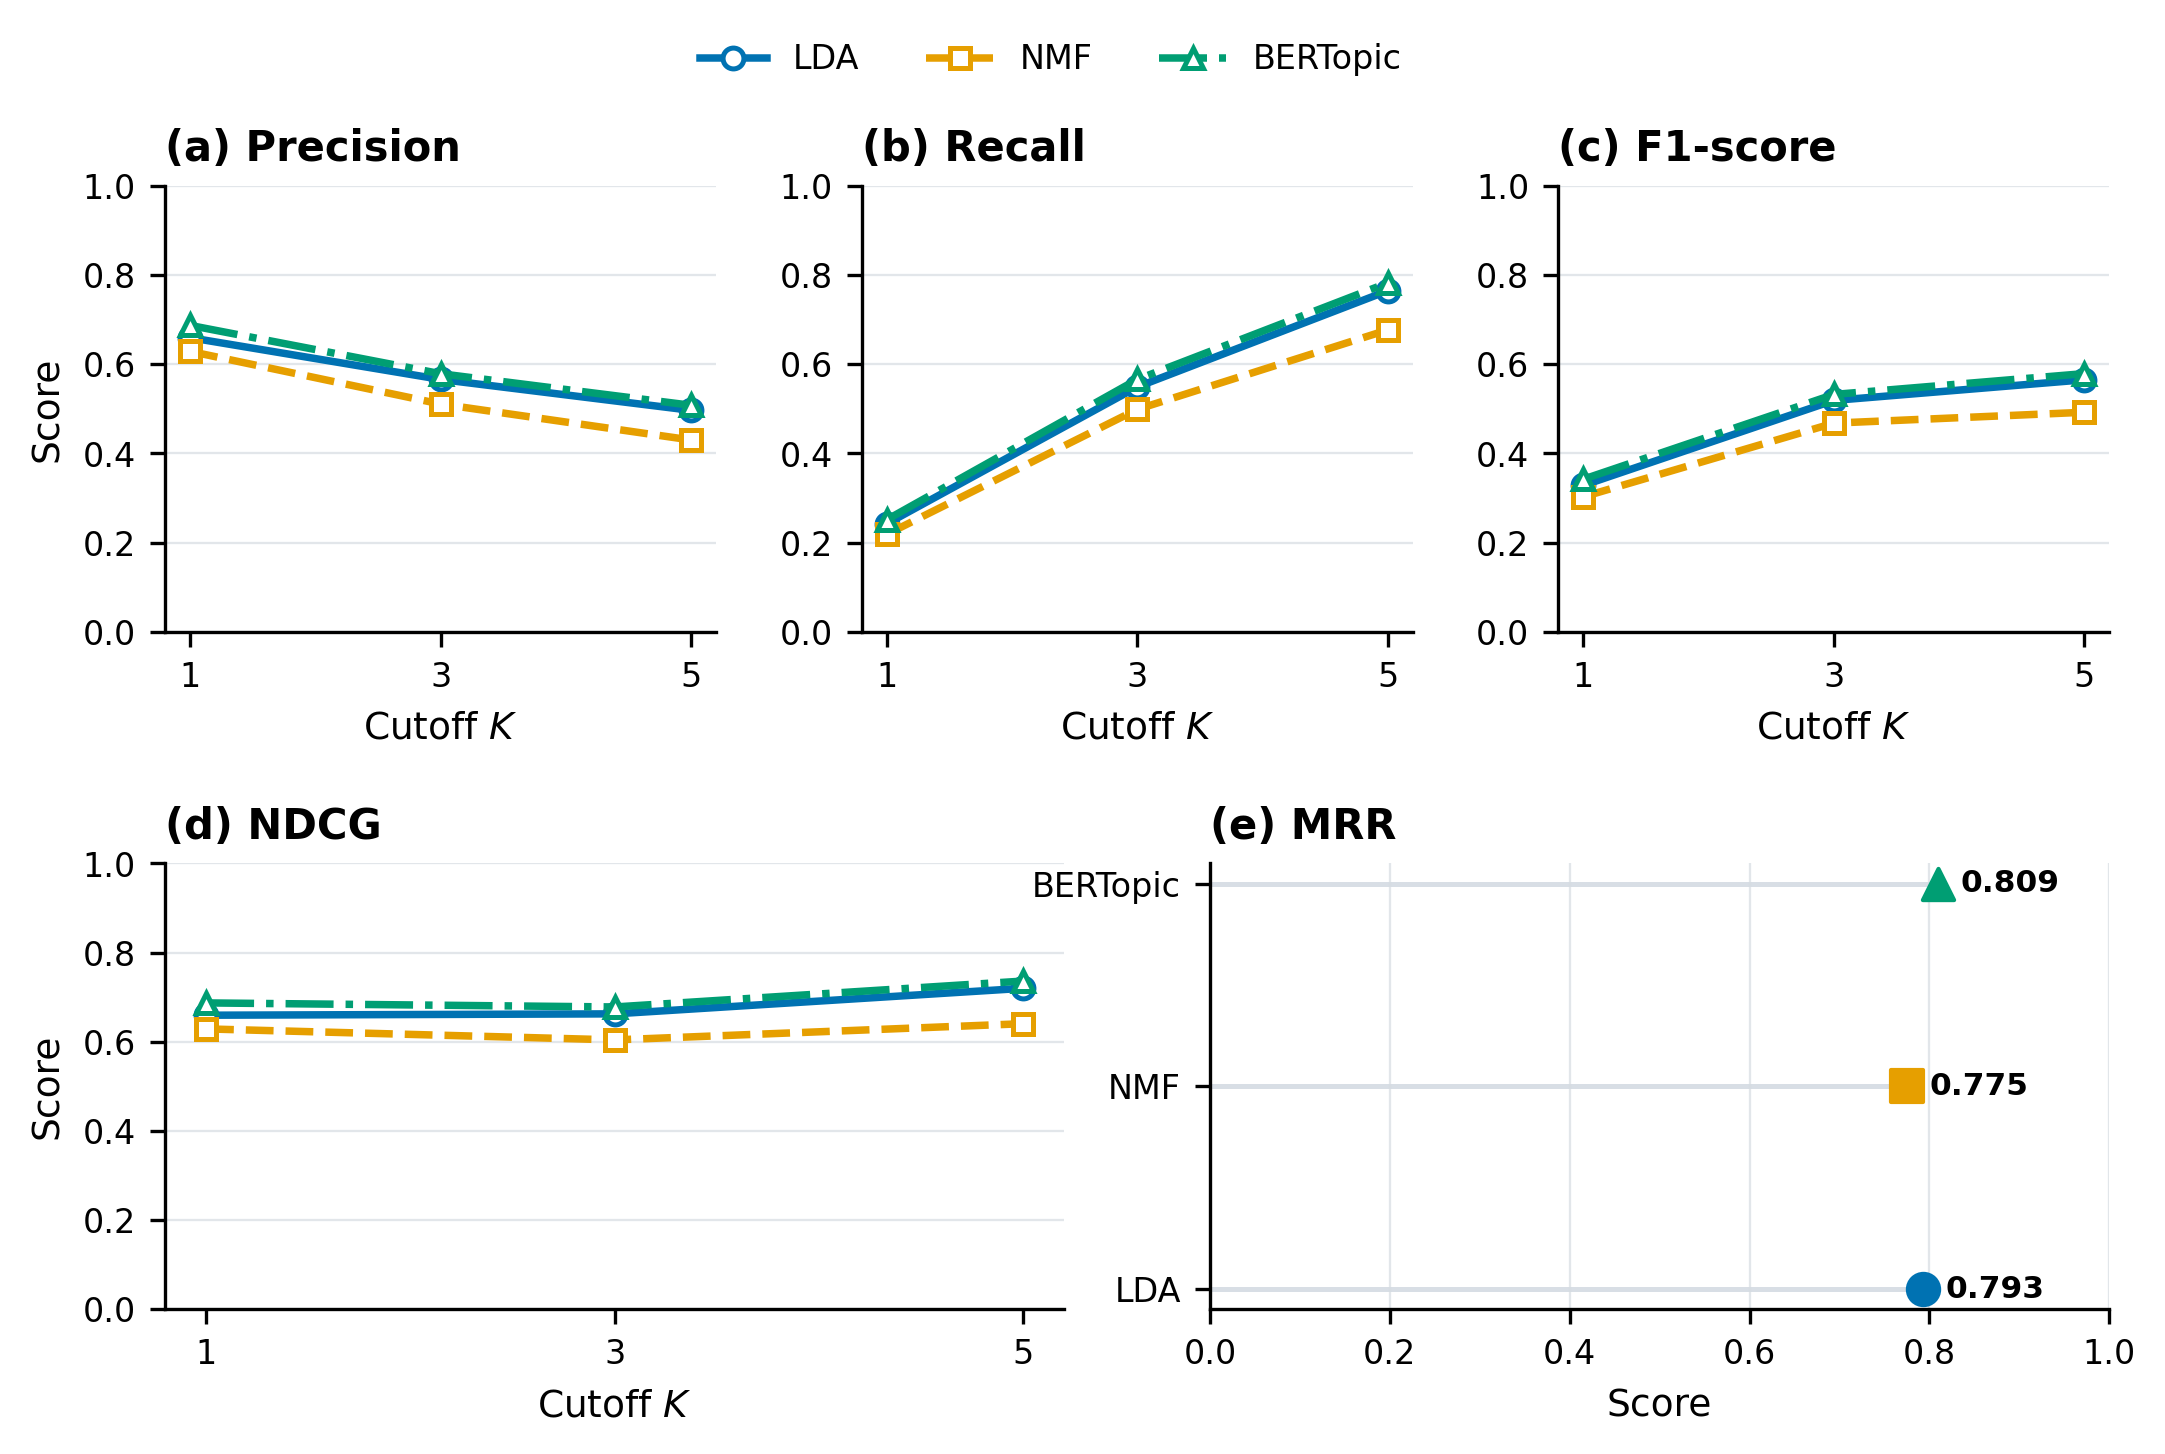
\includegraphics[width=0.94\columnwidth]{sections/figures/04_recommendation_performance.png}
    \caption{Recommendation performance.}
    \label{fig:recperf}
\end{figure}

BERTopic's advantage over NMF was statistically significant for every tested metric, surviving the Bonferroni-corrected threshold; its advantage over LDA was smaller, reaching nominal significance ($p<0.05$) only for Recall@5 and F1@5, with none of the five comparisons surviving Bonferroni correction. Across the complete set of 13 metrics, BERTopic differed significantly from LDA on 3 of 13 (23\%) and from NMF on 13 of 13 (100\%) at the uncorrected threshold: it ranks numerically first on every metric, but only its separation from NMF is statistically robust on this split, while its separation from LDA is a consistent yet comparatively fragile signal.

BERTopic's advantage may relate to its SPECTER embeddings, which represent scientific publications in a contextual semantic space that keeps related publications close even across different terms. Unlike LDA and NMF, fitted only on the roughly 11,000-document training corpus, SPECTER was pretrained on a much larger external corpus of scientific publications, so part of BERTopic's advantage may reflect this external pretraining signal rather than the topic-modeling mechanism itself; the experiment did not isolate the embedding, dimensionality-reduction, clustering, and outlier-reassignment components, so the difference cannot be assigned to one component alone.

\subsection{Topic Quality and Computational Runtime}
Fig.~\ref{fig:quality}(a) compared the final topic coherence values: NMF was highest (0.686782), followed by BERTopic (0.659480) and LDA (0.521625) -- an order that differs from the recommendation results, where NMF ranked last and BERTopic best despite the second-highest coherence. This mismatch suggests that $C_v$, which evaluates co-occurrence of leading words, and recommendation quality, which depends on whether complete topic vectors separate researcher and group profiles after aggregation, measure different properties; a model can produce coherent topic words without the most useful ranking representation, consistent with prior evidence that intrinsic topic metrics do not always predict downstream performance~\cite{rudiger2022topic}.

Runtime (Fig.~\ref{fig:quality}(b)) also differed substantially: NMF was fastest (18.1~s training, 0.7~s inference), LDA required 178.5~s/1.8~s, and BERTopic 966.5~s/5.2~s, for total execution times of 18.8~s, 180.3~s, and 971.8~s respectively (unrounded per-stage totals can differ by up to 0.1~s from the one-decimal figures above, e.g.\ BERTopic's 971.777~s rounds to 971.8~s though 966.5~s+5.2~s sums to 971.7~s). Training accounted for most of the measured time for every model.

\begin{figure}[t]
    \centering
    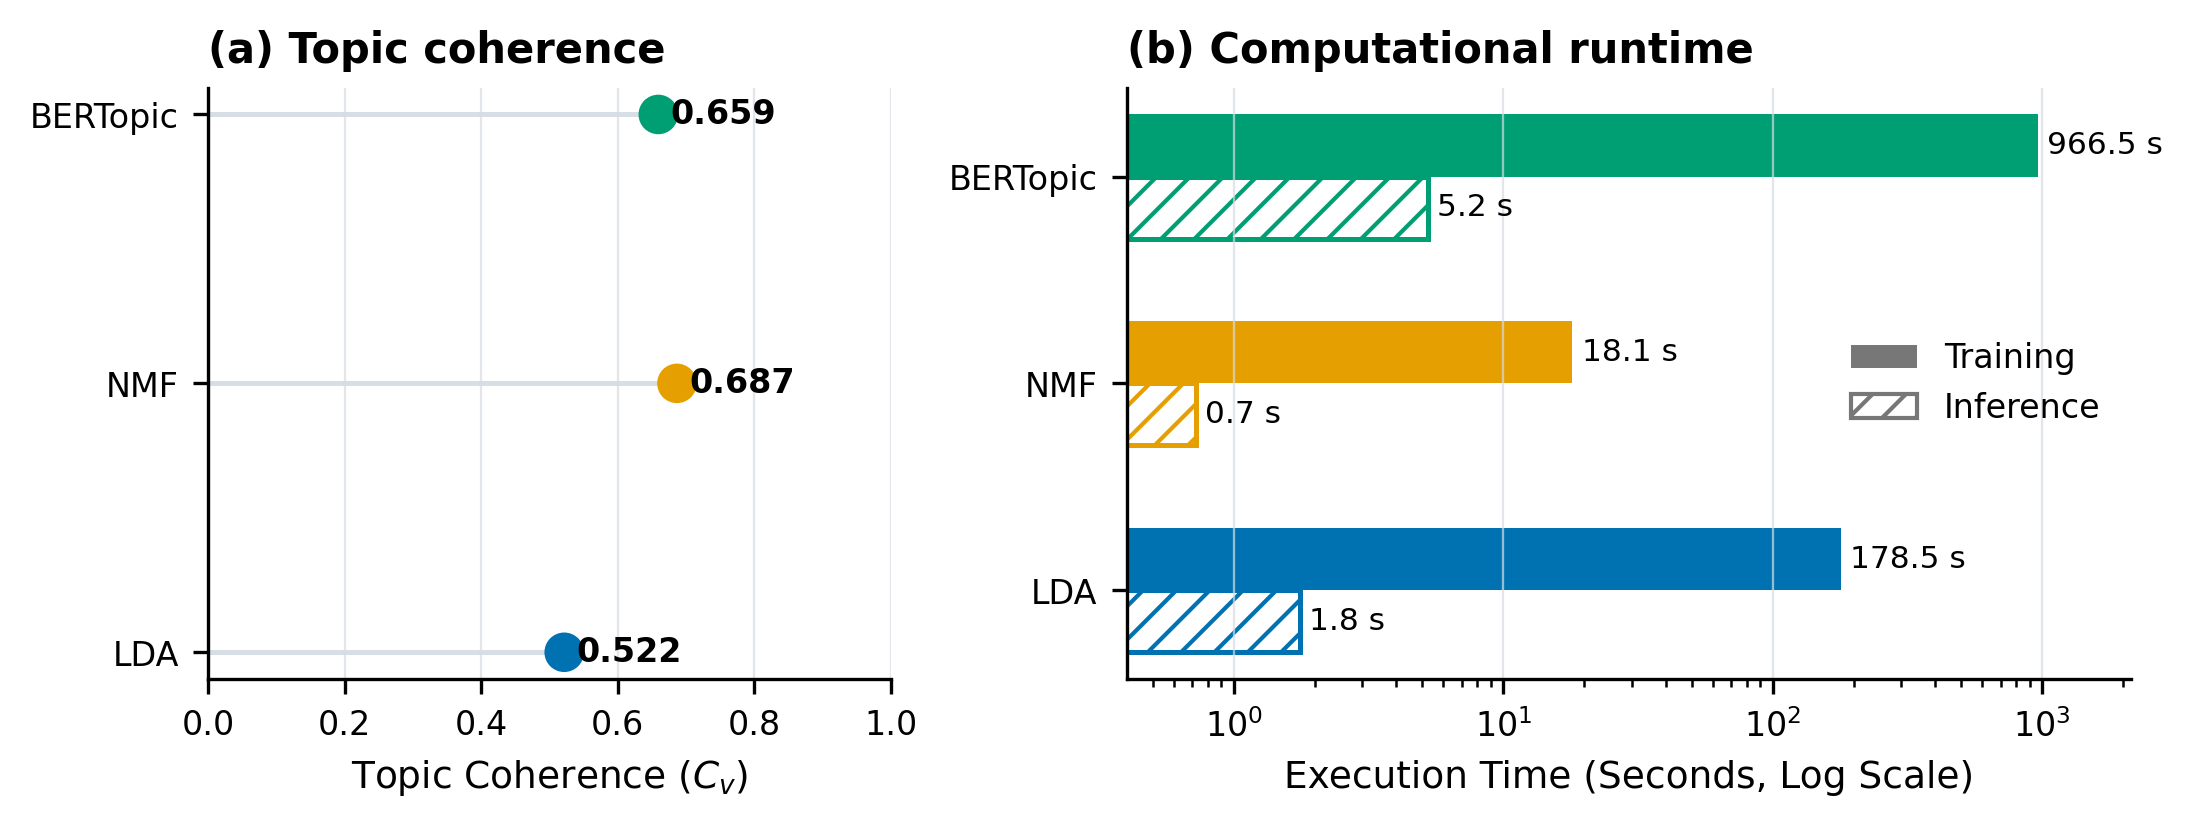
\includegraphics[width=0.94\columnwidth]{sections/figures/05_model_quality_and_runtime.png}
    \caption{Model characteristics: (a) topic coherence and (b) computational runtime.}
    \label{fig:quality}
\end{figure}

This pattern shows a clear quality/cost trade-off: BERTopic is preferable when ranking accuracy has priority and training can run offline, NMF when frequent retraining or limited resources matter, and LDA occupies a middle position with quality close to BERTopic at lower cost. Hardware and dependency-version details for this run were not recorded, so these figures should be read as indicative of relative model cost rather than an absolute, reproducible benchmark.

\subsection{Performance Across Research Groups}
Fig.~\ref{fig:pergroup} reported Top-3 precision per research group; performance varied more across groups than across models within a group. Machine Learning and Computer Vision had the highest values (approximately 0.91 and 0.86--0.89), followed by Artificial Intelligence and Natural Language Processing (0.63--0.74). The middle and lower rows showed wider separation: BERTopic led The Web and Information Retrieval (0.59), Databases (0.54), and Human-Computer Interaction (0.44); NMF led Robotics (0.60) and Data Mining (0.44); LDA led Natural Language Processing (0.74). No model ranked first for every group: counting the highest or tied-highest score across the 12 groups, BERTopic led in 6 (including a tie with LDA in Machine Learning), LDA in 4, and NMF in 3.

\begin{figure}[t]
    \centering
    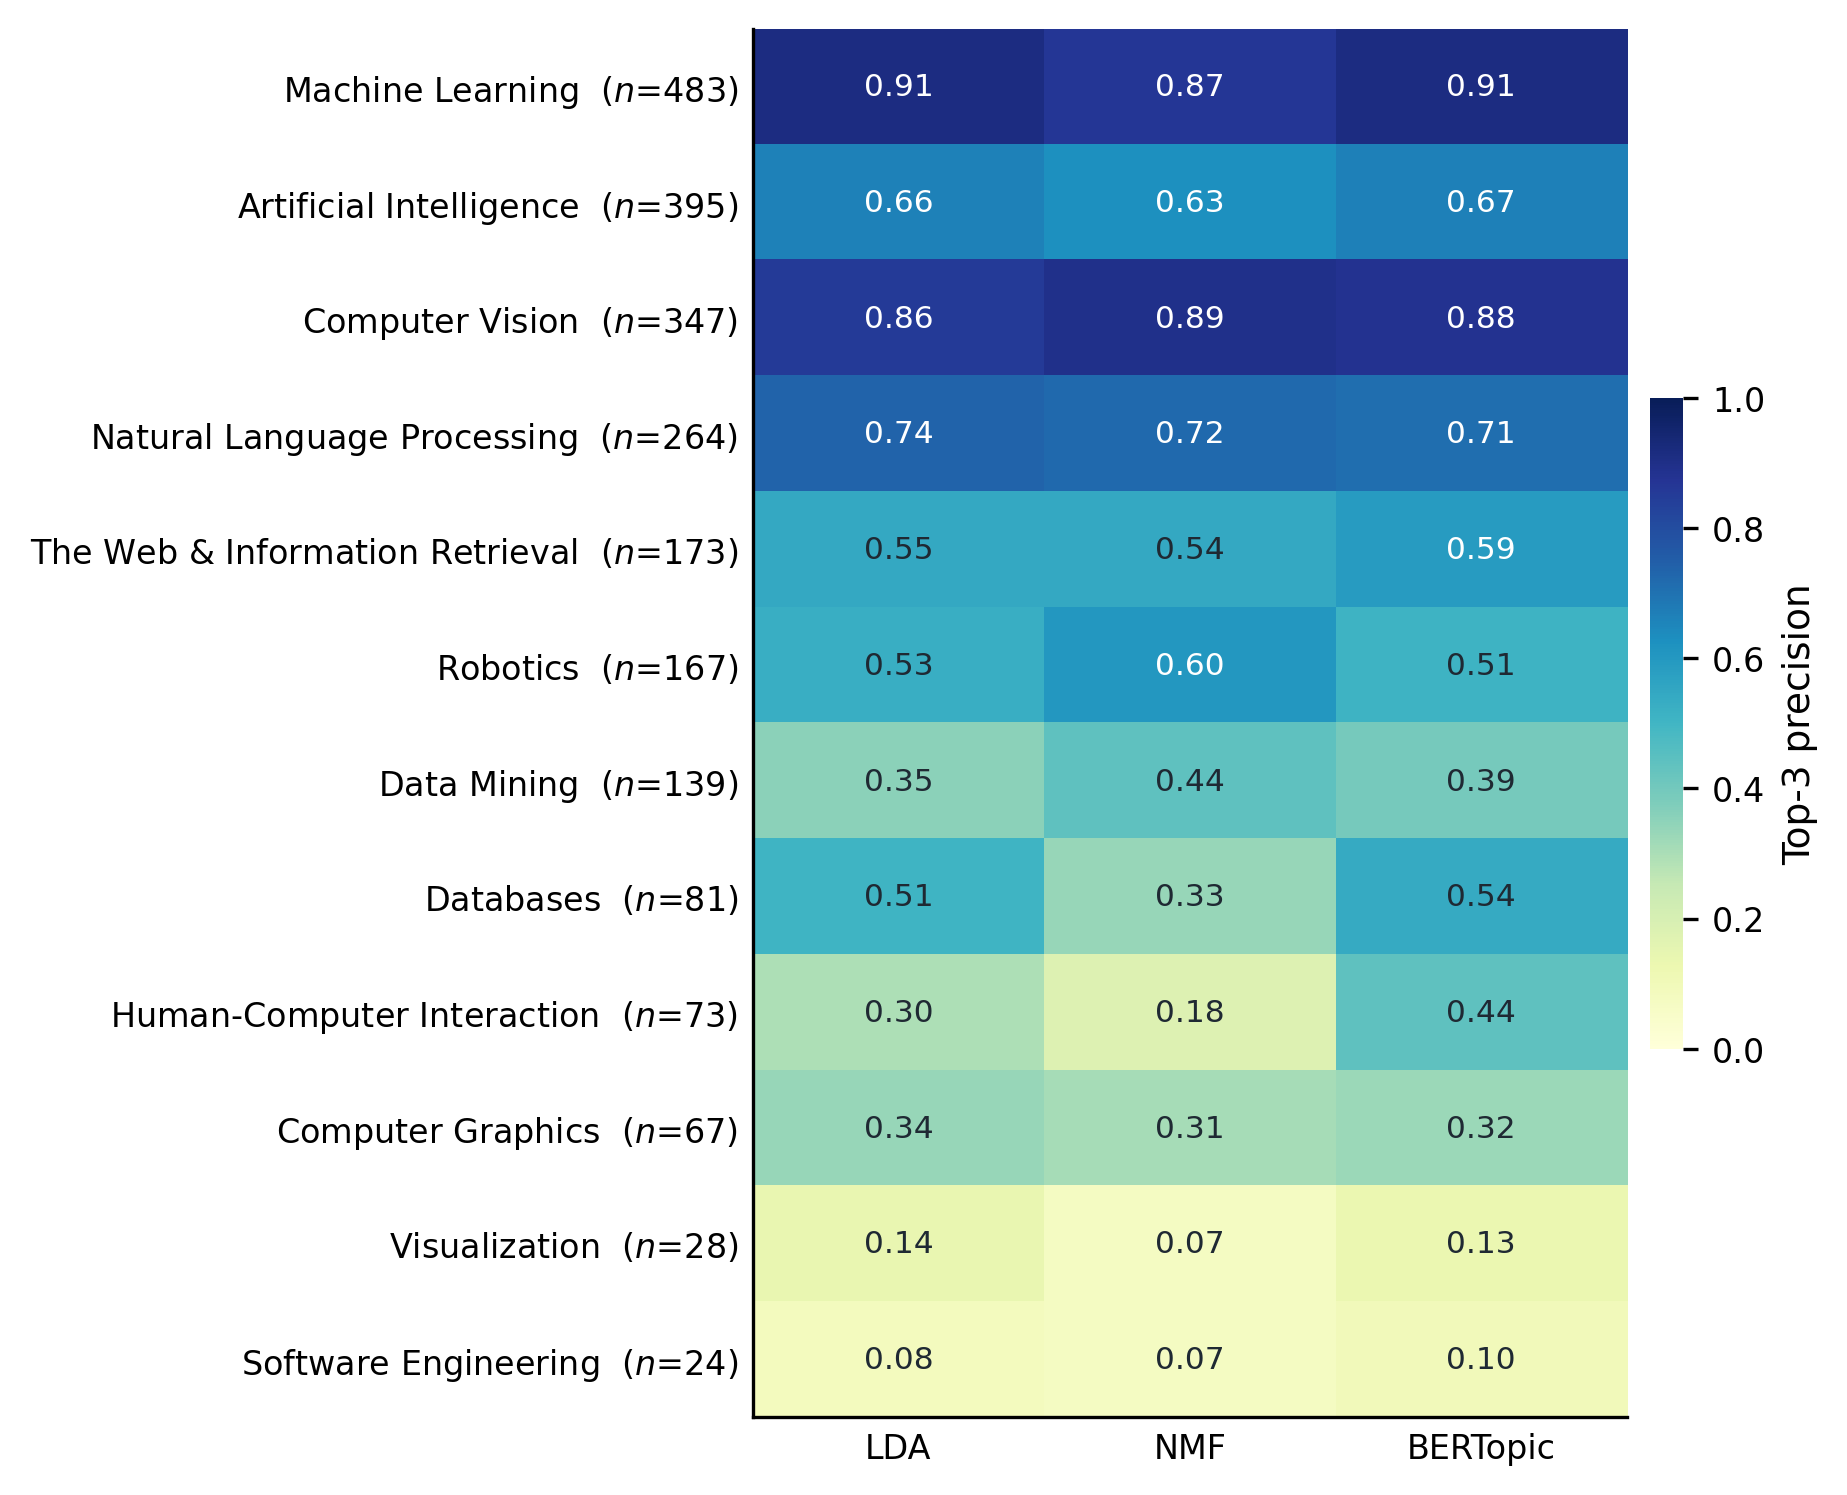
\includegraphics[width=0.94\columnwidth]{sections/figures/06_per_group_performance.png}
    \caption{Top-3 precision by research group.}
    \label{fig:pergroup}
\end{figure}

The smallest test groups recorded the lowest Top-3 precision: Visualization ($n=28$) scored 0.07--0.14 and Software Engineering ($n=24$) scored 0.07--0.10, while Computer Graphics stayed below 0.34 despite 67 relevant researchers; Databases, by contrast, reached 0.54 with BERTopic from 81 researchers, so group size alone did not explain the differences. Because Top-3 precision is a proportion from a small sample, its variability is largest where the group is smallest: a binomial standard error of $\sqrt{p(1-p)/n} \approx 0.05\text{--}0.06$ around a precision near 0.10 for Visualization and Software Engineering implies a 95\% confidence interval spanning most of the observed range, so their model orderings should be read as indicative rather than conclusive.
